\definecolor{pp}{RGB}{127,201,127}
\definecolor{cc}{RGB}{0,0,0}
\definecolor{oo}{RGB}{251,128,114}

% GNUPLOT: LaTeX picture with Postscript
\begingroup
  \makeatletter
  \providecommand\color[2][]{%
    \GenericError{(gnuplot) \space\space\space\@spaces}{%
      Package color not loaded in conjunction with
      terminal option `colourtext'%
    }{See the gnuplot documentation for explanation.%
    }{Either use 'blacktext' in gnuplot or load the package
      color.sty in LaTeX.}%
    \renewcommand\color[2][]{}%
  }%
  \providecommand\includegraphics[2][]{%
    \GenericError{(gnuplot) \space\space\space\@spaces}{%
      Package graphicx or graphics not loaded%
    }{See the gnuplot documentation for explanation.%
    }{The gnuplot epslatex terminal needs graphicx.sty or graphics.sty.}%
    \renewcommand\includegraphics[2][]{}%
  }%
  \providecommand\rotatebox[2]{#2}%
  \@ifundefined{ifGPcolor}{%
    \newif\ifGPcolor
    \GPcolorfalse
  }{}%
  \@ifundefined{ifGPblacktext}{%
    \newif\ifGPblacktext
    \GPblacktexttrue
  }{}%
  % define a \g@addto@macro without @ in the name:
  \let\gplgaddtomacro\g@addto@macro
  % define empty templates for all commands taking text:
  \gdef\gplfronttext{}%
  \gdef\gplfronttext{}%
  \makeatother
  \ifGPblacktext
    % no textcolor at all
    \def\colorrgb#1{}%
    \def\colorgray#1{}%
  \else
    % gray or color?
    \ifGPcolor
      \def\colorrgb#1{\color[rgb]{#1}}%
      \def\colorgray#1{\color[gray]{#1}}%
      \expandafter\def\csname LTw\endcsname{\color{white}}%
      \expandafter\def\csname LTb\endcsname{\color{black}}%
      \expandafter\def\csname LTa\endcsname{\color{black}}%
      \expandafter\def\csname LT0\endcsname{\color[rgb]{1,0,0}}%
      \expandafter\def\csname LT1\endcsname{\color[rgb]{0,1,0}}%
      \expandafter\def\csname LT2\endcsname{\color[rgb]{0,0,1}}%
      \expandafter\def\csname LT3\endcsname{\color[rgb]{1,0,1}}%
      \expandafter\def\csname LT4\endcsname{\color[rgb]{0,1,1}}%
      \expandafter\def\csname LT5\endcsname{\color[rgb]{1,1,0}}%
      \expandafter\def\csname LT6\endcsname{\color[rgb]{0,0,0}}%
      \expandafter\def\csname LT7\endcsname{\color[rgb]{1,0.3,0}}%
      \expandafter\def\csname LT8\endcsname{\color[rgb]{0.5,0.5,0.5}}%
    \else
      % gray
      \def\colorrgb#1{\color{black}}%
      \def\colorgray#1{\color[gray]{#1}}%
      \expandafter\def\csname LTw\endcsname{\color{white}}%
      \expandafter\def\csname LTb\endcsname{\color{black}}%
      \expandafter\def\csname LTa\endcsname{\color{black}}%
      \expandafter\def\csname LT0\endcsname{\color{black}}%
      \expandafter\def\csname LT1\endcsname{\color{black}}%
      \expandafter\def\csname LT2\endcsname{\color{black}}%
      \expandafter\def\csname LT3\endcsname{\color{black}}%
      \expandafter\def\csname LT4\endcsname{\color{black}}%
      \expandafter\def\csname LT5\endcsname{\color{black}}%
      \expandafter\def\csname LT6\endcsname{\color{black}}%
      \expandafter\def\csname LT7\endcsname{\color{black}}%
      \expandafter\def\csname LT8\endcsname{\color{black}}%
    \fi
  \fi
    \setlength{\unitlength}{0.0500bp}%
    \ifx\gptboxheight\undefined%
      \newlength{\gptboxheight}%
      \newlength{\gptboxwidth}%
      \newsavebox{\gptboxtext}%
    \fi%
    \setlength{\fboxrule}{0.5pt}%
    \setlength{\fboxsep}{1pt}%
\begin{picture}(8000.00,8000.00)%
    \gplgaddtomacro\gplfronttext{%
    }%
    \gplgaddtomacro\gplfronttext{%
      \colorrgb{0.00,0.00,0.00}%
      \put(3999,7959){\makebox(0,0){\strut{}\small Αρχική συνθήκη}}%
      \put(600, 3770){\makebox(0,0){\strut{}{\color{pp}{\rule[0.6mm]{0.5cm}{0.5mm}}} \small Σφάλμα θέσης [m]}}
      \put(3420,3770){\makebox(0,0){\strut{}{\color{oo}{\rule[0.6mm]{0.5cm}{0.5mm}}} \small Σφάλμα προσανατολισμού [rad]}}
      \put(7020,3770){\makebox(0,0){\strut{}{\color{cc}{\rule[0.6mm]{0.5cm}{0.5mm}}} \small Οικεία εσωτερική μετρική σφάλματος [m]}}
    }%
    \gplgaddtomacro\gplfronttext{%
    }%
    \gplgaddtomacro\gplfronttext{%
      \colorrgb{0.00,0.00,0.00}%
      \put(1839,5959){\makebox(0,0){\strut{}\small Εξέλιξη ευθυγράμμισης FastGICP}}%
    }%
    \gplgaddtomacro\gplfronttext{%
    }%
    \gplgaddtomacro\gplfronttext{%
      \colorrgb{0.00,0.00,0.00}%
      \put(6159,5959){\makebox(0,0){\strut{}\small Εξέλιξη ευθυγράμμισης \texttt{fsm}}}%
    }%
    \gplgaddtomacro\gplfronttext{%
      \colorrgb{0.00,0.45,0.74}%
      \put(508,2400){\makebox(0,0)[r]{\strut{}\scriptsize $0.0$}}%
      \colorrgb{0.00,0.45,0.74}%
      \put(508,2543){\makebox(0,0)[r]{\strut{}\scriptsize $0.2$}}%
      \colorrgb{0.00,0.45,0.74}%
      \put(508,2685){\makebox(0,0)[r]{\strut{}\scriptsize $0.4$}}%
      \colorrgb{0.00,0.45,0.74}%
      \put(508,2828){\makebox(0,0)[r]{\strut{}\scriptsize $0.6$}}%
      \colorrgb{0.00,0.45,0.74}%
      \put(508,2971){\makebox(0,0)[r]{\strut{}\scriptsize $0.8$}}%
      \colorrgb{0.00,0.45,0.74}%
      \put(508,3114){\makebox(0,0)[r]{\strut{}\scriptsize $1.0$}}%
      \colorrgb{0.00,0.45,0.74}%
      \put(508,3256){\makebox(0,0)[r]{\strut{}\scriptsize $1.2$}}%
      \colorrgb{0.00,0.45,0.74}%
      \put(508,3399){\makebox(0,0)[r]{\strut{}\scriptsize $1.4$}}%
    }%
    \gplgaddtomacro\gplfronttext{%
    }%
    \gplgaddtomacro\gplfronttext{%
      \colorrgb{0.15,0.15,0.15}%
      \put(640,2180){\makebox(0,0){\strut{}\scriptsize $0$}}%
      \colorrgb{0.15,0.15,0.15}%
      \put(1089,2180){\makebox(0,0){\strut{}\scriptsize $10$}}%
      \colorrgb{0.15,0.15,0.15}%
      \put(1538,2180){\makebox(0,0){\strut{}\scriptsize $20$}}%
      \colorrgb{0.85,0.33,0.10}%
      \put(1715,2400){\makebox(0,0)[l]{\strut{}}}%
      \colorrgb{0.85,0.33,0.10}%
      \put(1715,2600){\makebox(0,0)[l]{\strut{}}}%
      \colorrgb{0.85,0.33,0.10}%
      \put(1715,2800){\makebox(0,0)[l]{\strut{}}}%
      \colorrgb{0.85,0.33,0.10}%
      \put(1715,2999){\makebox(0,0)[l]{\strut{}}}%
      \colorrgb{0.85,0.33,0.10}%
      \put(1715,3199){\makebox(0,0)[l]{\strut{}}}%
      \colorrgb{0.85,0.33,0.10}%
      \put(1715,3399){\makebox(0,0)[l]{\strut{}}}%
    }%
    \gplgaddtomacro\gplfronttext{%
    }%
    \gplgaddtomacro\gplfronttext{%
      \colorrgb{1.00,0.00,1.00}%
      \put(2108,2400){\makebox(0,0)[r]{\strut{}\scriptsize $0$}}%
      \colorrgb{1.00,0.00,1.00}%
      \put(2108,2574){\makebox(0,0)[r]{\strut{}\scriptsize $0.18$}}%
      \colorrgb{1.00,0.00,1.00}%
      \put(2108,2749){\makebox(0,0)[r]{\strut{}\scriptsize $0.35$}}%
      \colorrgb{1.00,0.00,1.00}%
      \put(2108,2923){\makebox(0,0)[r]{\strut{}\scriptsize $0.52$}}%
      \colorrgb{1.00,0.00,1.00}%
      \put(2108,3097){\makebox(0,0)[r]{\strut{}\scriptsize $0.70$}}%
      \colorrgb{1.00,0.00,1.00}%
      \put(2108,3272){\makebox(0,0)[r]{\strut{}\scriptsize $0.87$}}%
    }%
    \gplgaddtomacro\gplfronttext{%
    }%
    \gplgaddtomacro\gplfronttext{%
      \colorrgb{0.15,0.15,0.15}%
      \put(2240,2180){\makebox(0,0){\strut{}\scriptsize $0$}}%
      \colorrgb{0.15,0.15,0.15}%
      \put(2689,2180){\makebox(0,0){\strut{}\scriptsize $10$}}%
      \colorrgb{0.15,0.15,0.15}%
      \put(3138,2180){\makebox(0,0){\strut{}\scriptsize $20$}}%
      \colorrgb{0.85,0.33,0.10}%
      \put(3315,2400){\makebox(0,0)[l]{\strut{}\scriptsize $0$}}%
      \colorrgb{0.85,0.33,0.10}%
      \put(3315,2600){\makebox(0,0)[l]{\strut{}\scriptsize $100$}}%
      \colorrgb{0.85,0.33,0.10}%
      \put(3315,2800){\makebox(0,0)[l]{\strut{}\scriptsize $200$}}%
      \colorrgb{0.85,0.33,0.10}%
      \put(3315,2999){\makebox(0,0)[l]{\strut{}\scriptsize $300$}}%
      \colorrgb{0.85,0.33,0.10}%
      \put(3315,3199){\makebox(0,0)[l]{\strut{}\scriptsize $400$}}%
      \colorrgb{0.85,0.33,0.10}%
      \put(3315,3399){\makebox(0,0)[l]{\strut{}\scriptsize $500$}}%
    }%
    \gplgaddtomacro\gplfronttext{%
    }%
    \gplgaddtomacro\gplfronttext{%
      \colorrgb{0.00,0.45,0.74}%
      \put(4668,2400){\makebox(0,0)[r]{\strut{}\scriptsize $0.0$}}%
      \colorrgb{0.00,0.45,0.74}%
      \put(4668,2650){\makebox(0,0)[r]{\strut{}\scriptsize $0.1$}}%
      \colorrgb{0.00,0.45,0.74}%
      \put(4668,2900){\makebox(0,0)[r]{\strut{}\scriptsize $0.2$}}%
      \colorrgb{0.00,0.45,0.74}%
      \put(4668,3149){\makebox(0,0)[r]{\strut{}\scriptsize $0.3$}}%
      \colorrgb{0.00,0.45,0.74}%
      \put(4668,3399){\makebox(0,0)[r]{\strut{}\scriptsize $0.4$}}%
    }%
    \gplgaddtomacro\gplfronttext{%
    }%
    \gplgaddtomacro\gplfronttext{%
      \colorrgb{0.15,0.15,0.15}%
      \put(5010,2180){\makebox(0,0){\strut{}\scriptsize $2$}}%
      \colorrgb{0.15,0.15,0.15}%
      \put(5219,2180){\makebox(0,0){\strut{}\scriptsize $4$}}%
      \colorrgb{0.15,0.15,0.15}%
      \put(5429,2180){\makebox(0,0){\strut{}\scriptsize $6$}}%
      \colorrgb{0.15,0.15,0.15}%
      \put(5638,2180){\makebox(0,0){\strut{}\scriptsize $8$}}%
      \colorrgb{0.85,0.33,0.10}%
      \put(5875,2400){\makebox(0,0)[l]{\strut{}}}%
      \colorrgb{0.85,0.33,0.10}%
      \put(5875,2650){\makebox(0,0)[l]{\strut{}}}%
      \colorrgb{0.85,0.33,0.10}%
      \put(5875,2900){\makebox(0,0)[l]{\strut{}}}%
      \colorrgb{0.85,0.33,0.10}%
      \put(5875,3149){\makebox(0,0)[l]{\strut{}}}%
      \colorrgb{0.85,0.33,0.10}%
      \put(5875,3399){\makebox(0,0)[l]{\strut{}}}%
    }%
    \gplgaddtomacro\gplfronttext{%
    }%
    \gplgaddtomacro\gplfronttext{%
      \colorrgb{1.00,0.00,1.00}%
      \colorrgb{1.00,0.00,1.00}%
      \put(6268,2400){\makebox(0,0)[r]{\strut{}\scriptsize $0$}}%
      \colorrgb{1.00,0.00,1.00}%
      \put(6268,2574){\makebox(0,0)[r]{\strut{}\scriptsize $0.18$}}%
      \colorrgb{1.00,0.00,1.00}%
      \put(6268,2749){\makebox(0,0)[r]{\strut{}\scriptsize $0.35$}}%
      \colorrgb{1.00,0.00,1.00}%
      \put(6268,2923){\makebox(0,0)[r]{\strut{}\scriptsize $0.52$}}%
      \colorrgb{1.00,0.00,1.00}%
      \put(6268,3097){\makebox(0,0)[r]{\strut{}\scriptsize $0.70$}}%
      \colorrgb{1.00,0.00,1.00}%
      \put(6268,3272){\makebox(0,0)[r]{\strut{}\scriptsize $0.87$}}%
    }%
    \gplgaddtomacro\gplfronttext{%
    }%
    \gplgaddtomacro\gplfronttext{%
      \colorrgb{0.15,0.15,0.15}%
      \put(6610,2180){\makebox(0,0){\strut{}\scriptsize $2$}}%
      \colorrgb{0.15,0.15,0.15}%
      \put(6819,2180){\makebox(0,0){\strut{}\scriptsize $4$}}%
      \colorrgb{0.15,0.15,0.15}%
      \put(7029,2180){\makebox(0,0){\strut{}\scriptsize $6$}}%
      \colorrgb{0.15,0.15,0.15}%
      \put(7238,2180){\makebox(0,0){\strut{}\scriptsize $8$}}%
      \colorrgb{0.85,0.33,0.10}%
      \put(7475,2400){\makebox(0,0)[l]{\strut{}\scriptsize $0$}}%
      \colorrgb{0.85,0.33,0.10}%
      \put(7475,2650){\makebox(0,0)[l]{\strut{}\scriptsize $50$}}%
      \colorrgb{0.85,0.33,0.10}%
      \put(7475,2900){\makebox(0,0)[l]{\strut{}\scriptsize $100$}}%
      \colorrgb{0.85,0.33,0.10}%
      \put(7475,3149){\makebox(0,0)[l]{\strut{}\scriptsize $150$}}%
      \colorrgb{0.85,0.33,0.10}%
      \put(7475,3399){\makebox(0,0)[l]{\strut{}\scriptsize $200$}}%
    }%
    \gplgaddtomacro\gplfronttext{%
    }%
    \gplgaddtomacro\gplfronttext{%
    }%
    \gplgaddtomacro\gplfronttext{%
      \colorrgb{0.00,0.00,0.00}%
      \put(1839,1799){\makebox(0,0){\strut{}\small Τελική ευθυγράμμιση FastGICP}}%
    }%
    \gplgaddtomacro\gplfronttext{%
    }%
    \gplgaddtomacro\gplfronttext{%
      \colorrgb{0.00,0.00,0.00}%
      \put(6159,1799){\makebox(0,0){\strut{}\small Τελική ευθυγράμμιση \texttt{fsm}}}%
    }%
    \put(0,0){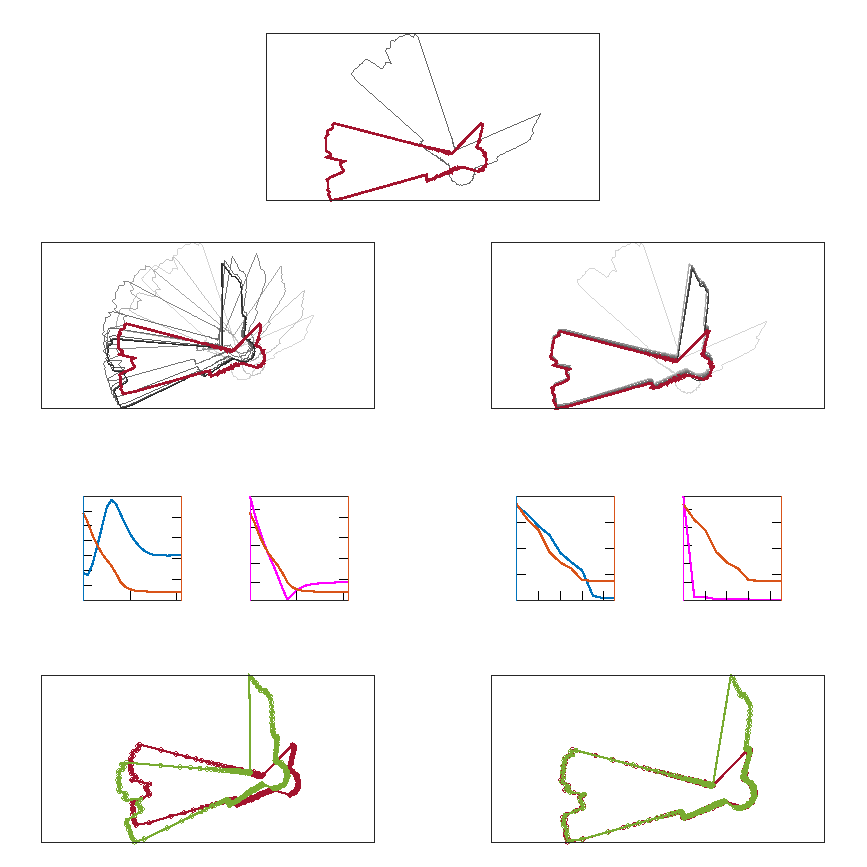
\includegraphics{./figures/parts/02/chapters/05/sections/04/fsm_vs_fgi}}%
    \gplfronttext
  \end{picture}%
\endgroup
